% !TEX root = ../master.tex
\chapter{Design}
\label{chap:design}

\section{Analysis of Cluster Environment}

The Hadoop cluster will be installed on the cluster computer at the \ac{DHBW} Mannheim.
This cluster utilizes \emph{OpenStack} to provide resources to its users. 
OpenStack is an open source project to manage public and private cloud computing architectures \autocite[][]{openstack}. 
It enables the compositions of compute elements (virtual machines), network elements (sub-nets and routers), 
and storage elements (virtual disks) to form a virtual computing environment.
The OpenStack management web interface can be accesses from within the \ac{DHBW} network. 
The \emph{Cloud Computing Competence Center} at the \ac{DHBW} Mannheim  manages the cluster computer \autocite[][]{dhbwmannheim20184c}.

The OpenStack environment is shared between multiple user groups, 
which each is given a certain amount of resources. 
For this project the student group is given a limited amount of resources.
Only 20 virtual \ac{CPU} cores, 50 \ac{GB} \ac{RAM} and 1 \ac{TB} of storage are dedicated to the project.
This resources can be used to allocate instances of \acp{VM} in pre-defined units and assign virtual disks to them.
The \acp{VM} can be connected to the network of the \ac{DHBW} and can be interconnected using internal, virtual networks.
Firewall restrictions can be set through group policies, which can be assigned to the \acp{VM}. 
When creating a new \ac{VM} most of these settings must be supplied. 
Furthermore the operating system flavour can be chosen and a \ac{SSH} login key can be provided.
Among others \emph{Ubuntu Server 16.04 LTS} can be used which is compatible with Hadoop in general.

The Hadoop cluster be deployed on multiple interconnected \acp{VM} in the OpenStack environment that can be accessed from the university network.

The connection to the \ac{DHBW} network gives some restrictions: \acp{VM} can only be accessed from the university network and not from the Internet.
From a security point of view this decreases potential attack vectors.
However for development access it is restricting, 
since the developer needs to be on premise. 

\section{Analysis of Requirements}

There are three main user groups that can be determined for the Hadoop cluster:

\begin{itemize}
    \item \textbf{IT Staff} -- The technical staff at the \ac{DHBW} can perform maintenance on the Hadoop cluster and possibly a re-setup of it.
    Also they might use it for research projects.
    \item \textbf{Lecturers} -- Lecturers might most likely use the cluster for the purpose of teaching classes about \ac{BDA} and give hands on experiences for the students. They might prepare the educational material and data sets on the cluster and exemplary demonstrate its usage.
    \item \textbf{Students} -- Students at the \ac{DHBW} might use the cluster within the context of courses or research project to perform data analysis. Within lectures they might be instructed by the teacher, in research project they can use the cluster on their own.
\end{itemize}

In his paper, \emph{Philipp Winter} discusses more possible use cases for the cluster. It focuses on the educational usability in lectures.
Main users are lecturers and students to perform analytics of various data on the cluster.

Sicklinger et al. also did a requirements analysis for an Hadoop cluster at the \ac{DHBW}. 
\begin{itemize}
    \item The cluster utilizes the OpenStack Environment in Mannheim.
    \item There should be only a low cost, at best no cost, associated with deploying and running the cluster.
    \item It should be possible for students and lecturers to deploy the cluster.
    \item The cluster should provide the ability to be used to learn about the Hadoop deployment and learn about data analysis.
    \item The it should support recent tools to be used alongside with Hadoop.
    \item The cluster should scale to the needs of the users.
\end{itemize}
\autocite[][p. 40ff]{wi2018managementsystems}


All of the listed requirements imply that the cluster needs to be deployable without extended or expert knowledge about Hadoop itself.
Automated deployment is therefore favourable to make the procedure reproducible. 
Still it can be required for the person performing the installation to have general knowledge about system administration on Linux based machines.


\section{Research on Possibilities}

After the requirements are settled,
the possibilities of how Hadoop can be installed 
on the given infrastructure will be researched. Therefore first a understanding how Hadoop clusters can be deployed and maintained more efficiently using \emph{Cluster Management Systems} is established.
Then possible ways to install Hadoop are evaluated experimentally and features and drawbacks of each approach are laid out.
This will lead to an decision on the method that should be used for the cluster at the \ac{DHBW}.

\subsubsection{Cluster Management Systems}
\label{sec:design:clustermanagement}
To deploy Hadoop on an cluster there are two general approaches. Either the Hadoop distribution package is installed and configured manually on each node or an management tool is used to perform automatic deployment and configuration. 
Since the manual installation process is error prone (as visible in section \ref{sec:design:manualinstall}) and needs some know-how,
it is  more easy for the user to utilize an management system for the cluster.

The management system can provide, install, manage and monitor software components on the cluster nodes.
Not only \ac{HDFS} and \ac{YARN} can be deployed,
but also additional tools can be integrated into the cluster this way.
Usually the management system also provides an graphical user interface to perform those tasks.

To provide the components the management system downloads them from a given binary distribution repository. The installation can be performed via remote access from the management server to the nodes. Monitoring gives valuable information to the cluster user, such as capacity an utilization of computational power and storage.

\subsubsection{Hadoop Distributions}
Some vendors choose to bundle a management system 
together with an specific version of Hadoop and additional Tools. They offer this bundle mostly as binary packages which are considered \emph{distributions} of Hadoop.
For system maintainers this holds the benefit that no compilation from source is necessary and the versions of the tools are adjusted to work with each other. 
Notable distributions are \emph{\acf{CDH}} and \emph{\acf{HDP}}. 

There are four ways to install Hadoop that are considered here:

\begin{itemize}
    \item A \emph{manual installation} of Hadoop 
        and every additional piece of software from the ecosystem
    \item \emph{\acf{CDH}} --  An open source software distribution by Cloudera including Hadoop
        and additional software from the ecosystem
        \urlinline{https://www.cloudera.com/products/open-source/apache-hadoop/key-cdh-components.html}
    \item \emph{Ambari} -- An open source project by Apache that provides
        the capability to manage Hadoop Clusters and the software components running on it.
        \urlinline{https://ambari.apache.org/}
    \item \emph{\acf{HDP}} -- Hortonswork's ready-to-install distribution of Hadoop 
        with Ambari and additional software
        \urlinline{https://de.hortonworks.com/products/data-platforms/hdp/}
    \item \emph{MapR} -- Commercial Hadoop distribution by MapR Data Technologies, Inc. A community edition is available. \urlinline{https://mapr.com/}
        
\end{itemize}

Since \ac{HDP} makes use of Ambari for installing the cluster and managing the installed software \autocite[][]{hortonworks2018ambari} while it simply provides a pre-packaged version of the components, 
it can be preferred over using Ambari directly which would create the need to compile it from source.

\emph{MapR} will not be discussed, since its free-of-charge community edition is only permitted to be used for \enquote{[internal] trial, evaluation, testing or similar non-production purposes} \autocite[][para.~1.5]{mapr2018EULA}. 
It therefore does not qualify to be used permanently at the \ac{DHBW} for educational purposes.

In the next sections the remaining three options, 
\emph{manual installation, \ac{CDH} and \ac{HDP}}
are tested and compared by performing a exemplary installation.
Each of the evaluations considers the complexity and susceptibility to error of the installation process.


\subsubsection{Evaluation Environment}
In the coming sections each of those three resulting possibilities will be looked at in more detail.
For each of the options an evaluation will be made on whether it is 
feasible to deploy an Hadoop installation with the methods that they provide.
Therefore a simple test installation in an OpenStack environment is made.
For this purpose the OpenStack environment \emph{BWCloud} \urlinline{https://www.bw-cloud.org/de/projekt}
is used, an environment that is available for students at the \ac{DHBW} 
and other universities in Baden-Württemberg for educational purposes. 
It is generally an equivalent software to the actual cluster environment, 
however it is accessible from the Internet, 
which makes it more comfortable to work with while performing the tests.

\subsection{Manual Installation of Hadoop}
\label{sec:design:manualinstall}

The first possibility to install Hadoop onto a number of hosts 
is to use the installation package provided by Apache them self \urlinline{https://hadoop.apache.org/releases.html}.
This represents the most basic procedure of installation.
Tom White \autocite[][Appendix A]{white2015hadoop} describes how Hadoop can be manually installed on the machines in an cluster. 
Manually here means without the help of automated installers for a single machine or the complete cluster. 
Every aspect of the installation and configuration must be done \enquote{by hand}.
White gives step by step instruction on the process.

Since no step in this step is predetermined or automated, this method does not really install an "Hadoop distribution" on the cluster, but rather only \ac{YARN}, \ac{HDFS} and MapReduce.
It does not provide a \emph{management system} for Hadoop.

\subsubsection{System Setup}
For the installation two \acs{VM} are used, utilizing two virtual \ac{CPU} cores and eight \ac{GB} \ac{RAM} and a 20 \ac{GB} storage drive. 
Ubuntu Serve 16.04.3 \ac{LTS} is used as the operating system. 
The machines are connected to the public Internet and to each other using two network interfaces each.

The two machines are going to be connected together in an master-slave setup
where the master runs the \ac{YARN} resource manager and the \ac{HDFS} name node as well as an \ac{HDFS} data node and an \ac{YARN} client node.
The slaves runs only an \ac{HDFS} data node and an \ac{YARN} client node.

First the system of the master is configured. Therefore the following steps are taken.

\begin{enumerate}
    \item The system is updated and OpenJDK 1.8 \urlinline{http://openjdk.java.net/}  is installed using \texttt{apt}. 
    \item A new user \emph{hadoop} is created which will be used to run every service on the machine concerning Hadoop.
    \item For this user a new \ac{SSH} key is created which enables password-less access to the two machines for the user \emph{hadoop} if its public key is later added to the \texttt{authorized\_key} file of the user on the hosts.
    \item The \texttt{/etc/hosts} file is adjusted, such that both hosts know how to reach each other on the local network by using their \acs{FQDN} which is resolved to an \ac{IP} address.
    \item The network interface to the internal network that is connected is configured to use the \ac{IP} address assigned to it by OpenStack.
    \item \ac{IP}v6 is disabled.
\end{enumerate}

The slave system uses mainly the same configuration but is altered slightly.
No new \ac{SSH} key is generated, but the public key of the previously
generated one is entered into the \texttt{authorized\_key} file. 
Furthermore an additional 70 \ac{GB} hard drive is attached 
and mounted to store working data.

After the base system is configured, Hadoop can be installed on both machines
and can be configured to form a cluster.
Again, first the master host is configured.
Therefore the next steps describes in 
\autocite[][Appendix A]{white2015hadoop}
can be followed.

\begin{enumerate}
    \item First Hadoop is downloaded from the Apache website \urlinline{https://hadoop.apache.org/releases.html}. 
    At the moment of performing this tests, 
    version 2.7.4 is the latest stable release.
    The downloaded packed file is unzipped in the home directory of the \emph{hadoop} user.
    \item Inside the \texttt{bashrc} file of the user the the variables \texttt{JAVA\_HOME} is pointing to the OpenJDK installation,
    \texttt{HADOOP\_HOME} is set to the folder that has just been crated and the \texttt{PATH} variable is configured to include the \texttt{bin} directory within \texttt{HADOOP\_HOME}.
    Each variable is exported to be available in the user shell.
    This makes Hadoop usable from the login shell of the user.
    \item Now the configuration files of Hadoop are adjusted to the cluster needs. Each of those resides in the \texttt{etc/hadoop} directory within \texttt{HADOOP\_HOME}.
    \begin{itemize}
        \item \texttt{core-site.xml} -- This file describes the most basic settings for the instaled Hadoop instance. 
        Here the settings for the file system is set to use the \ac{FQDN} of the master to connect to.
        \item \texttt{hadoop-env.sh} -- This file describes all the environment variables used while running Hadoop. 
        Here \texttt{JAVA\_HOME} is set to the same value used above.
        \item \texttt{hdfs-site.xml} -- This file describes how \ac{HDFS} is configured. 
        The storage directory is set to a persistent folder
        and \ac{HDFS} is instructed to bind to the \ac{IP} address 0.0.0.0 
        which means the file system is accessible from all network interfaces.
        \item \texttt{mapred-site.xml} -- Here the settings for MapReduce are made. 
        It is instructed to use \ac{YARN} as the underlying framework.
        \item \texttt{slaves} -- This file is used on the master host to identify all the hosts 
        that run an NodeManager or an DataNode.
        Therefore the \acs{FQDN} of the master and the salve host are entered here.
        \item \texttt{yarn-site.xml} -- This file describes the settings for \ac{YARN}. Here the master's \ac{FQDN} is entered as the ResourceManager and \ac{YARN} is bound to 0.0.0.0. 
        Furthermore the minimal allocation units for \ac{CPU} cores 
        as well as \ac{RAM} and their respective maximum allocation are defined. 
        This dictates how \ac{YARN} uses the resources of this host.
    \end{itemize}
\end{enumerate}

After the configuration is done for the master host, the same procedure can be followed for the slave. 
The only exceptions are that no entries are made in the \texttt{slaves} file 
and the \texttt{hdfs-site.xml} is configured, so that \ac{HDFS} uses the attached data drive to store file contents.

Finally the \ac{HDFS} file systems on each host can be formatted to initialize the \ac{HDFS} storage.
Then \ac{YARN} and \ac{HDFS}, as well as the MapReduce history server is started on the master, 
which in turn start the NameNode and resoucemanager on the master 
as well as the DataNode and NodeManager on both the master and the slave.
Now the cluster can be used to store data in \ac{HDFS} and run MapReduce jobs.

\subsubsection{Tests}
\autocite[][]{white2015hadoop} provides an online reference (http://hadoopbook.com/)
to test data and MapReduce programs 
that can be used for demonstration purposes of the Hadoop cluster.
The provided data includes weather data produced by the \ac{NCDC} and programs that can be run on Hadoop to analyze this data. 
Storing this data in \ac{HDFS} and running the MapReduce jobs lead to the discovery of erroneous configurations in the cluster.

Further test included the execution \emph{teragen} and \emph{terasort} \autocite[][]{omally2008terasort}, which generates a variable amount of numbers and sorts them, in this case 5 \ac{GB} of data. 
The generation  was successful, however the sorting failed due to an repeated connection timeout, which could not be resolved.

\subsubsection{Errors and Lessons Learned}
The whole described setup procedure is performed manually 
and therefore rather error prone.
Special attention to the usage of \acs{FQDN} must be given, 
so that the names used in Hadoop and the hostnames match up.
Those also need to be used in the \texttt{hosts} files on all hosts.

Furthermore it is important to configure the firewalls of OpenStack correctly, 
so that the nodes can be reached internally and externally.

Errors in the configuration lead to nodes that are not recognized by Hadoop or jobs that do not succeed.
It is rather frustrating to find and fix those issues for the person installing the cluster.

\subsubsection{Conclusions}

Due to the difficulties that the method of manually installing Hadoop on each host holds it is favorable to use a more streamlined 
and automated installation method as described in the next two sections.
This way a lot of manual configuration can be avoided.
Furthermore integrating tools such as Spark into the cluster 
will lead to even more complex installation and configuration processes which again might introduce new openings for errors.

\subsection{\acl{HDP} with Ambari deployed with Ansible}
\label{sec:design:hdp_ambari_ansible}
TODO describe HDP, Ambari,
eg \autocite[][]{hortonworks2018ambari}

The tested version of \ac{HDP} is 2.6.3.0 includes Ambari version 2.6.0.

\paragraph{Ansible}
\emph{Ansible} is an agent-less configuration management tool.
It ensures that the state of a computer system matches a desired and described state.
This includes operating system setting, service availability and configuration, 
as well as file contents and many more.
\enquote{Ansible uses \ac{YAML} files as its main source of information at run time. 
\ac{YAML} is a data representation language that is commonly used for configuration.
[...]
[It] is written entirely in Python [and it] works by running commands via \ac{SSH}, so there’s no need to install any server software.}
\autocite[][Chap. 1]{heap2016ansible}
The desired system configuration is descibed in a \emph{playbook}, 
which guides Ansible in the steps to apply this configuration.
A playbook can be split up into \emph{roles} to separate the configurations of different concerns.
Roles can be assigned to multiple hosts and can be combined if a hosts has multiple duties.
For the following test such a playbook is created.

Alternatives are \emph{Puppet} \autocite[][]{puppet} and \emph{Chef} \autocite[][]{chef} , which both use a central server to distribute the system configurations \autocite[][Chap. 1]{heap2016ansible}. 
This increases the complexity of the deployment setup.
Ansible avoids this and is therefore favourable for this test.

\subsubsection{System Setup}

As in the sections before the OpenStack BW-Cloud is used for a test deployment.
Three \acs{VM} are started, each with 20 \ac{GB} disk space, Ubuntu 16.04 \ac{LTS}, an public \ac{IP} address. 
The hosts are connected with an internal \ac{IP} network.
One \ac{VM} are used as the Ambari and Hadoop master node, having 2 virtual \ac{CPU} cores and 4 \ac{GB} \ac{RAM}.
Two \acs{VM} are used as slave nodes with 4 \acs{CPU} and 8 \ac{GB} \ac{RAM} as well as 2 \acs{CPU} and 4 \ac{GB} \ac{RAM} respectively.

Ansible is used to perform all system configuration. 
However before Ansible can be used, Python 2.7 needs to be installed on the hosts.
Now every deployed configuration is reproducible by running the Ansible configuration management again.
Hortonworks describes which steps of system setup are necessary 
to run Ambari when the installation is performed on a shell \autocite[][]{hortonworks2018install}.
The configuration using Ansible  performs the following similar steps:
\begin{enumerate}
    \item The internal network interfaces are configured 
        and the \texttt{\/etc\/hosts} file is filled with the hostnames 
        of all nodes and their integral \acs{IP}. 
        This prevents issues with the \ac{FQDN} resolution.
    \item The \ac{NTP} service is installed and started. 
        This is a requirement for Ambari.
    \item The \ac{THP}, a Linux kernel feature to improve memory look-ups, 
        is disabled using a service script. 
        This is a requirement for Ambari, 
        as it would reduce database performance.
        The script is based on \autocite{braun2017hugepages}.
    \item The Hortonworks Ambari repositories are added, so that the provided     binaries can be used.
    \item On the master \ac{VM} the Ambari server 
        and the Ambari agent is installed.
    \item On the slave nodes only the Ambari agent is installed.
    \item On the slave node the Ambari agent configuration is set to use the
        master node as its server.
    \item On the master node the initial Ambari server setup is performed which
        installs an \ac{JDK} 
        and starts the Ambari server service as the root user.
\end{enumerate}

Now the Hadoop cluster can be deployed using the Ambari Cluster Manager 
via an web interface on port 8080 on the master node, 
which needs to be accessible through the firewall of OpenStack.
Ambari provides an assisted install dialogue for the cluster installation. 
Here a new cluster deployment counting all three hosts is started.
The node need to be registered manually, as no shared \ac{SSH} key is present, that allows root access to the machines. 
(The web interface would require the used to upload the private key for root access, which is generally unsafe.)
The master node is configured to act as an Hadoop master and Hadoop salve. 
It is also the master for all recommended services running alongside of Hadoop.
The \emph{slaves} are salve machines for \ac{HDFS} and \ac{YARN}.
The cluster set-up dialogue then continues to install the cluster.


\subsection{Errors and Lessons Learned}
\label{sec:ambari:errors}
Since a lot of services such as Spark are recommended to be installed, 
the 20 \ac{GB} disk of the master is filled completely and the installation of the cluster fails. At least 50 \ac{GB} are recommended for an correct installation.
Therefore thee installation fails and the Hadoop deployment can not be functionally tested for now.

Ambari needs to be provided with the \ac{FQDN} of an host 
in all forms and configuration files. 
Otherwise it can not detect the agents or server.
The \acp{FQDN} must consist of at least to parts for Ambari to work with them. 
\emph{hadoop-master-0.dhbw} is valid, while \emph{hadoop-master-0} is not.

The Ambari clients need to be configured 
to use the correct Ambari server host.
Otherwise they will not be detected in the manual registration.

Furthermore using Ubuntu 16.04 might lead to problems, as \ac{HDP} explicitly supports Ubuntu 16.04 and 14.04 \autocite[][]{hortonworks2018requirements}, however Ambari only specifies compatibility to Ubuntu 12.04 and 14.04 \autocite[][]{ambari2018ambari}.


\subsubsection{Conclusions}
Ansible provides an reproducible way of system configuration 
and can therefore be used to install Ambari, 
which otherwise would require error-prone manual configuration on each host.
The Ambari Cluster Manager can then be used to install Hadoop and other services on the cluster with an user friendly web interface.


\subsection{\acl{CDH}}

Cloudera distributes an Hadoop management system called \ac{CDH} which makes use of \emph{Cloudera Manager} to deploy clusters.
\enquote{CDH is Cloudera’s 100\% open source platform distribution, including Apache Hadoop and built specifically to meet enterprise demands.}\autocite[][]{cloudera2018cdh}
It includes Hadoop and tools such as \emph{Apache HBase, Apache Hive, Apache Impala, Apache Kafka and Apache Spark}.
Cloudera provides an docker image which can be used to easily evaluate the usability of \ac{CDH}.
It contains \enquote{a single-host deployment of the Cloudera open-source distribution, including CDH and Cloudera Manager.} \autocite[][]{cloudera2018docker}
It does not provide a full cluster installation, but only a test environment to evaluate the platform that is contained inside the docker container.

It is important to note that using all features of \emph{Cloudera Manager} requires a paid license when installed on a cluster system. A 60 day trail version can also be obtained, which  \textcite[][p.~39]{wi2018managementsystems} point out, might be sufficient for usage at the \ac{DHBW}.

The tested version is \ac{CDH} 5.7.0 which can be obtained from \emph{DockerHub}, a repository for Docker container images.

\subsubsection{System Setup}

As in the previous section, BW-Cloud will be used for installing a test setup.
Since the Docker image only runs on a single host, this host should have as many resources as available in the testing environment.
Therefore the largest available \ac{VM} preset is used, which consists of 2 virtual \ac{CPU} cores, 
4 \ac{GB} \ac{RAM}, and 20 \ac{GB} storage. The operating is again Ubuntu 16.04 \ac{LTS}, 
and the host is accessible via the Internet. 
Cloudera describes how Docker can be installed and the test image can be started, 
these instructions are followed. \autocite[][]{cloudera2018docker}
To do so, the Docker runtime is installed, a new  user \emph{docker} is created and added to the \emph{docker} group. To test the Docker installation, the \emph{hello-world} image can be started.
Now all ports required by \ac{CDH} need to be accesible through the OpenStack firewall.
Namely these are 8888, 7080, and 8080 (which is used to redirect to port 80 inside the container).
After fetching the Docker  image, it can be started in daemon mode with the necessary ports exposed using the command\\
\texttt{\$ docker run --hostname=quickstart.cloudera --privileged=true -t -i -d -p 8888 -p 7080 -p 8080:80 cloudera/quickstart /usr/bin/docker-quickstart}\\
All services that are needed inside the container are started automatically.


\subsubsection{Tests}
The Docker image includes an web based tutorial, 
that can be accessed on port 8080 (remapped before) on the host.
The tutorial highlights the features of \ac{CDH} which differ from other Hadoop distributions.
The tutorial describes a story from the perspective of an data analyst and shows how the features provide value for typical use cases.

\subsubsection{Conclusions}
The tutorial provides a zero-configuration hands-on experience which focuses on the features specific to Cloudera's Hadoop distribution.
The installation inside the docker container seems stable.
However it is not possible to assume that this implies an error free installation on an cluster, 
since possible obstacles are not foreseeable.

\subsection{Decision on Distribution}
\label{sec:decision}

At this point it is important to mention the project paper by Sicklinger et al., 
who did research on the topic of the possible usage of Hadoop management systems for the \ac{DHBW}.
Their findings suggest using Apache Ambari to deploy an Hadoop cluster at the \ac{DHBW}.
According to them, installing Hadoop manually is ruled out due to the technical complexity.
Apache Ambari and Cloudera are equally suitable for the usage at the \ac{DHBW}, 
but Ambari should be favoured since it is free to use and crates no licensing costs.
\autocite[][p. 53f]{wi2018managementsystems}

In combination with Ansible, Ambari ensures an reproducible cluster installation. 
Therefore Ambari is the solution that will be used for this project and Ansible will be used to install the \ac{HDP} including Ambari.

\section{Architecture Design}

For the deployment of the Hadoop cluster, OpenStack will be used.
It provides the possibilities to create computational resources, which are \acs{VM}, 
storage resources, which are virtual disk volumes, 
and network resources, which are either project internal \ac{IP} networks or networks that are accessible from the outside of OpenStack.
With these resources it is possible to create an cluster that consists of interconnected nodes, 
that can store and process data and be accessed from the outside.

For this project a master-slave architecture is chosen.
Ambari promotes a sever-agent architecture, 
where the user can interact with Ambari on the server host 
and deploy the Hadoop cluster to all agent hosts.
Hadoop uses an cluster setup in which one server distributes and manages \ac{YARN} jobs (the \ac{YARN} ResourceManager), 
and keeps track of where data is stored data \ac{HDFS} (the \ac{HDFS} NameNode).
This can be considered a master.
To increase availability it is possible to choose a secondary master which replicates the \ac{HDFS} NameNode.
Figure \vref{fig:architecture} depicts the architecture that follows from these prerequisites.

\begin{figure}
	\fbox{
	    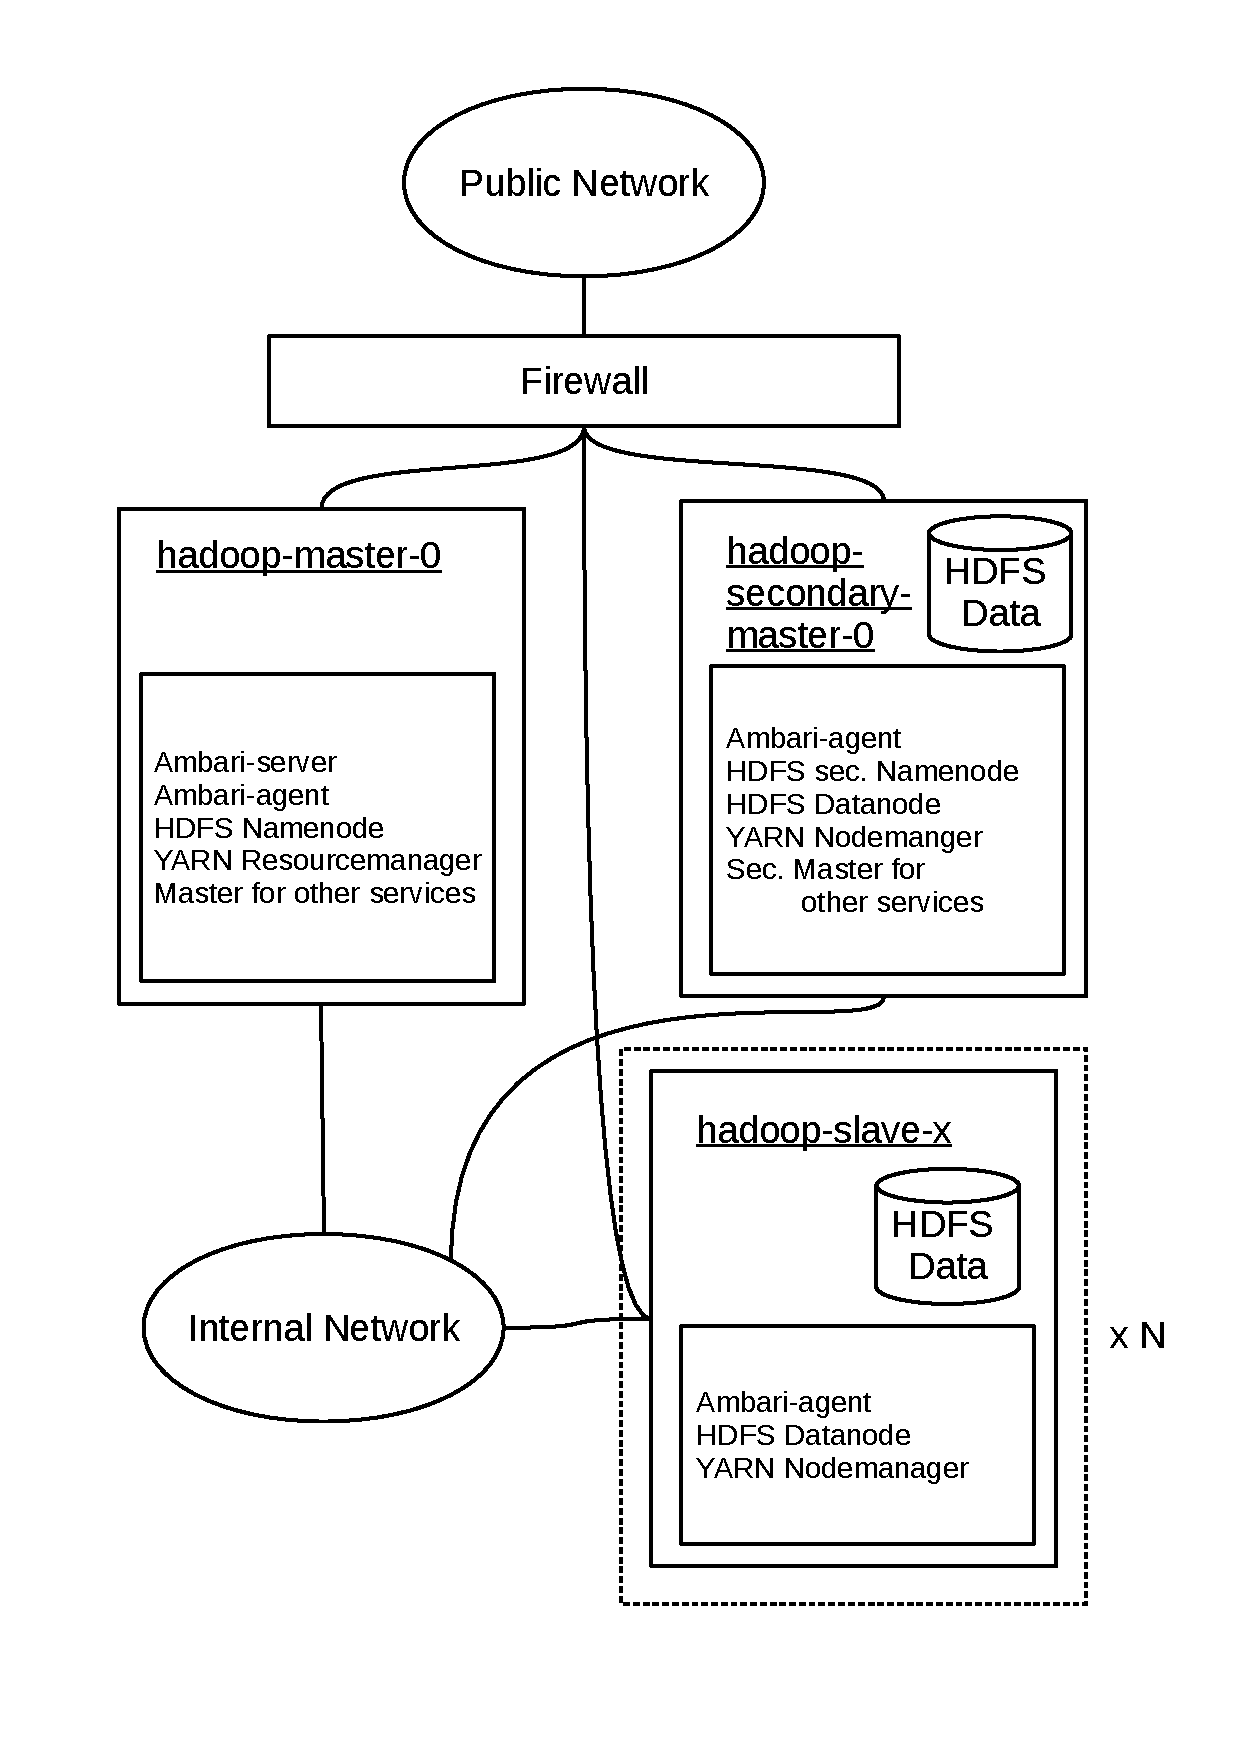
\includegraphics[width=\textwidth,height=\textheight,keepaspectratio]{resources/architecture.pdf}
    }
	\caption{\label{fig:architecture}Proposed Architecture}
\end{figure}

As discovered in section \vref{sec:ambari:errors} there should be at least 50 \ac{GB} of disk space on each node, 
just for Ambari and Hadoop to be installed.
For \ac{HDFS} data storage an additional volume should be attached to each of the \ac{HDFS} DataNodes.

The size of the used \acs{VM} should be the one with the most memory, 
as this is the resource where the overhead of having multiple \acs{VM} has the most impact.
All nodes need access to the Internet to download software packages and should be accessible via \ac{SSH} through the OpenStack firewall.
Furthermore the master node needs to be accessible via typical ports for the web interface of the deployed services and other ports which clients use to connect to the Hadoop cluster and issue jobs to it.
Internally all nodes need to be connected via an private network with fixed \acs{IP}, where the mapping between hostnames and \acs{IP} is known for each host. Typically this can be done with \ac{DNS}, however it is out of scope for this project to setup an \ac{DNS} server. Filling the \texttt{\/etc\/hosts} file is sufficient.
The internal network should not be restricted by any firewall.

Tom White recommends the following specification for a single node in a cluster, based on the needs of a full \ac{BDA} system in 2014:\\

\begin{itemize}
    \item Each node should run on dedicated, commodity hardware.
    \item Processor - Two hex/octo-core 3 GHz \acs{CPU}
    \item Memory 64 to 512 \ac{GB} \ac{ECC} \ac{RAM}
    \item Storage - 12 to 24 times 1 to 4 \ac{TB} disks
    \item Network - Gigabit Ethernet with link aggregation
\end{itemize}
\autocite{white2015hadoop}

However the given OpenStack environment does not allow the allocation of such amounts of resources, and has no possibility to use dedicated hardware. 
Therefore the maximum sized \acs{VM} should be used, and each be given an equal share of the available storage.

In case that it is only possible to allocate a small number of \acp{VM}, it can be useful to also assign the role of a DataNode and NodeManager to the master node. This allows the available resources on the master node not only to be used for management purposes but also for processing.

\section{Execution Plan}

In chapter \ref{chap:impl} the Hadoop cluster will be set up in an automated way.
To do so an execution plan is provided.
It functions as a reference to follow along during the implementation 
and can be used to reproduce the results in a similar way, i.e. to set up the cluster again in an similar environment.

In section \vref{sec:decision} the decision to use Apache Ambari in combination with Ansible has been made.
This scenario leads to the following steps regarding the deployment of the cluster into the OpenStack environment:

\begin{enumerate}
    \item \textbf{\ac{VM} Creation in OpenStack}
    As the first step, the host \acp{VM} need to be created in the OpenStack environment which will form the cluster.
    \begin{enumerate}
        \item Create an internal network.
        \item Create security groups which allow access with \ac{SSH}) to the hosts and via the web management portal to Ambari.
        \item Create an appropriate number of maximum sized \acp{VM} that are connected to both the internal and external network. Name them according to the names in \ref{fig:architecture}. Use a common domain, even if it is not officially registered. Provide some SSH credentials to log in.
        Assign the previously created security group to them.
        Ubuntu 14.04 or 16.04 should be used as the operating system.
        \item Note down the assigned internal and external \ac{IP} addresses displayed by OpenStack.
        \item Create virtual disks and assign them to the nodes. They will be used to store \ac{HDFS} data on them.
    \end{enumerate}
    
    \item \textbf{System Set-Up with Ansible} 
    In section \vref{sec:design:hdp_ambari_ansible} it has been shown that Ansible can be used to deploy \ac{HDP}. The Ansible playbook developed for this purpose can be adapted and used in the next steps.
    \begin{enumerate}
        %\item Configure the \texttt{ssh\_config} configuration file by supplying the \acp{FQDN} and the public \ac{IP} addresses of the nodes. 
        \item Configure the local \ac{SSH} client to use the \acp{FQDN} and the public \ac{IP} addresses of the nodes. 
        \item Check that all nodes can actually be accessed via \ac{SSH}
        \item Note down the name of the secondary (internal) Ethernet adapter of each node.
        \item Configure the Ansible inventory. Supply the internal \ac{IP} address as well as the previously noted Ethernet adapter of the node. he \emph{hadoop-master-0} node should be listed in the \emph{master} section, all others in the \emph{slave} section.
        \item Prepare the nodes for the usage with Ansible by installing Python on them and upgrading all system packages.
        \item Apply the Ansible playbook to the hosts.
        This configures the host systems in such a way that Ambari Server and Client respectively are installed on them.
    \end{enumerate}
    
    \item \textbf{Hadoop Set-Up with Ambari} 
    Next Hadoop itself, together with additional tools, can be deployed to the cluster using the Ambari cluster installation dialogue. This follows the instructions from \autocite[][Chap.~6]{hortonworks2018install}
    
    \begin{enumerate}
        \item Connect to Ambari via the web interface on the master node. The complete installation can be done from there.
        \item Ambari offers an cluster installation dialogue that firsts asks for all necessary configuration and checks it for consistency. The dialogue's instructions can be followed to deploy a cluster. 
        \item To select the hosts that should be included in the cluster, the \acp{FQDN} including a domain extension of all the \acp{VM} that have been created in the previous step should be provided.
        \item The \enquote{manual registration} option should be chosen, since otherwise an non-encrypted \ac{SSH} private key must be uploaded, which is unsafe.
        \item Next select the services and tools that should be included in the cluster installation. Hadoop is clearly mandatory, other tools that should be included are listed in \emph{Jonas Balsfullands' paper}. If Ambari detects unmet inter-dependencies, those should be corrected. 
        \item Assign the \emph{master} host to inhabit the master role in each service. If the service offers the possibility to register a secondary, fallback master this should be assigned to the \emph{secondary master} host.
        \item Assign slave nodes and clients to all of the nodes. This includes \emph{DataNodes} and \emph{NodeManager} and the Hadoop client tools.
        \item Configure all the services to the needs for the cluster. Most default settings can be kept. No service should depend on external resources such as existing databases. Set passwords to the services where needed. The passwords that have been set for each individual service should be documented. Ambari checks the settings for soundness and possibly warnings can be resolved manually.
        \item The installation then is being performed on the cluster. All selected components are installed with the selected configuration.
    \end{enumerate}
    
    \item \textbf{Test Usage} 
        To verify that the previous steps were successful, it is necessary to tests that the Hadoop cluster can be used
        \begin{enumerate}
            %\item Test that the master node can be reached from within the \ac{DHBW} network by connecting to it with a \ac{} and 
            
            % test connection to Hadoop master with hadoop client installed on workstation
            \item Test that \ac{HDFS} works by storing multiple, different sized files on the cluster file system.
            \item Test that MapReduce can be used to process data by running \emph{teragen} and \emph{terasort} on the cluster to create different amount of numbers and sort them. For example datasets with 100~\ac{MB}, 1~\ac{GB} and 5~\ac{GB} can be used for the tests.
        \end{enumerate}

\end{enumerate}

In the next chapter this execution plan will be implemented. More details about the technical solution and the exact execution, as well as the Ansible playbook will be given.


